\subsection{Results Part II: Preference Intensity Analysis}
\label{sec:result_2}

\begin{figure*}[h]
    \centering
    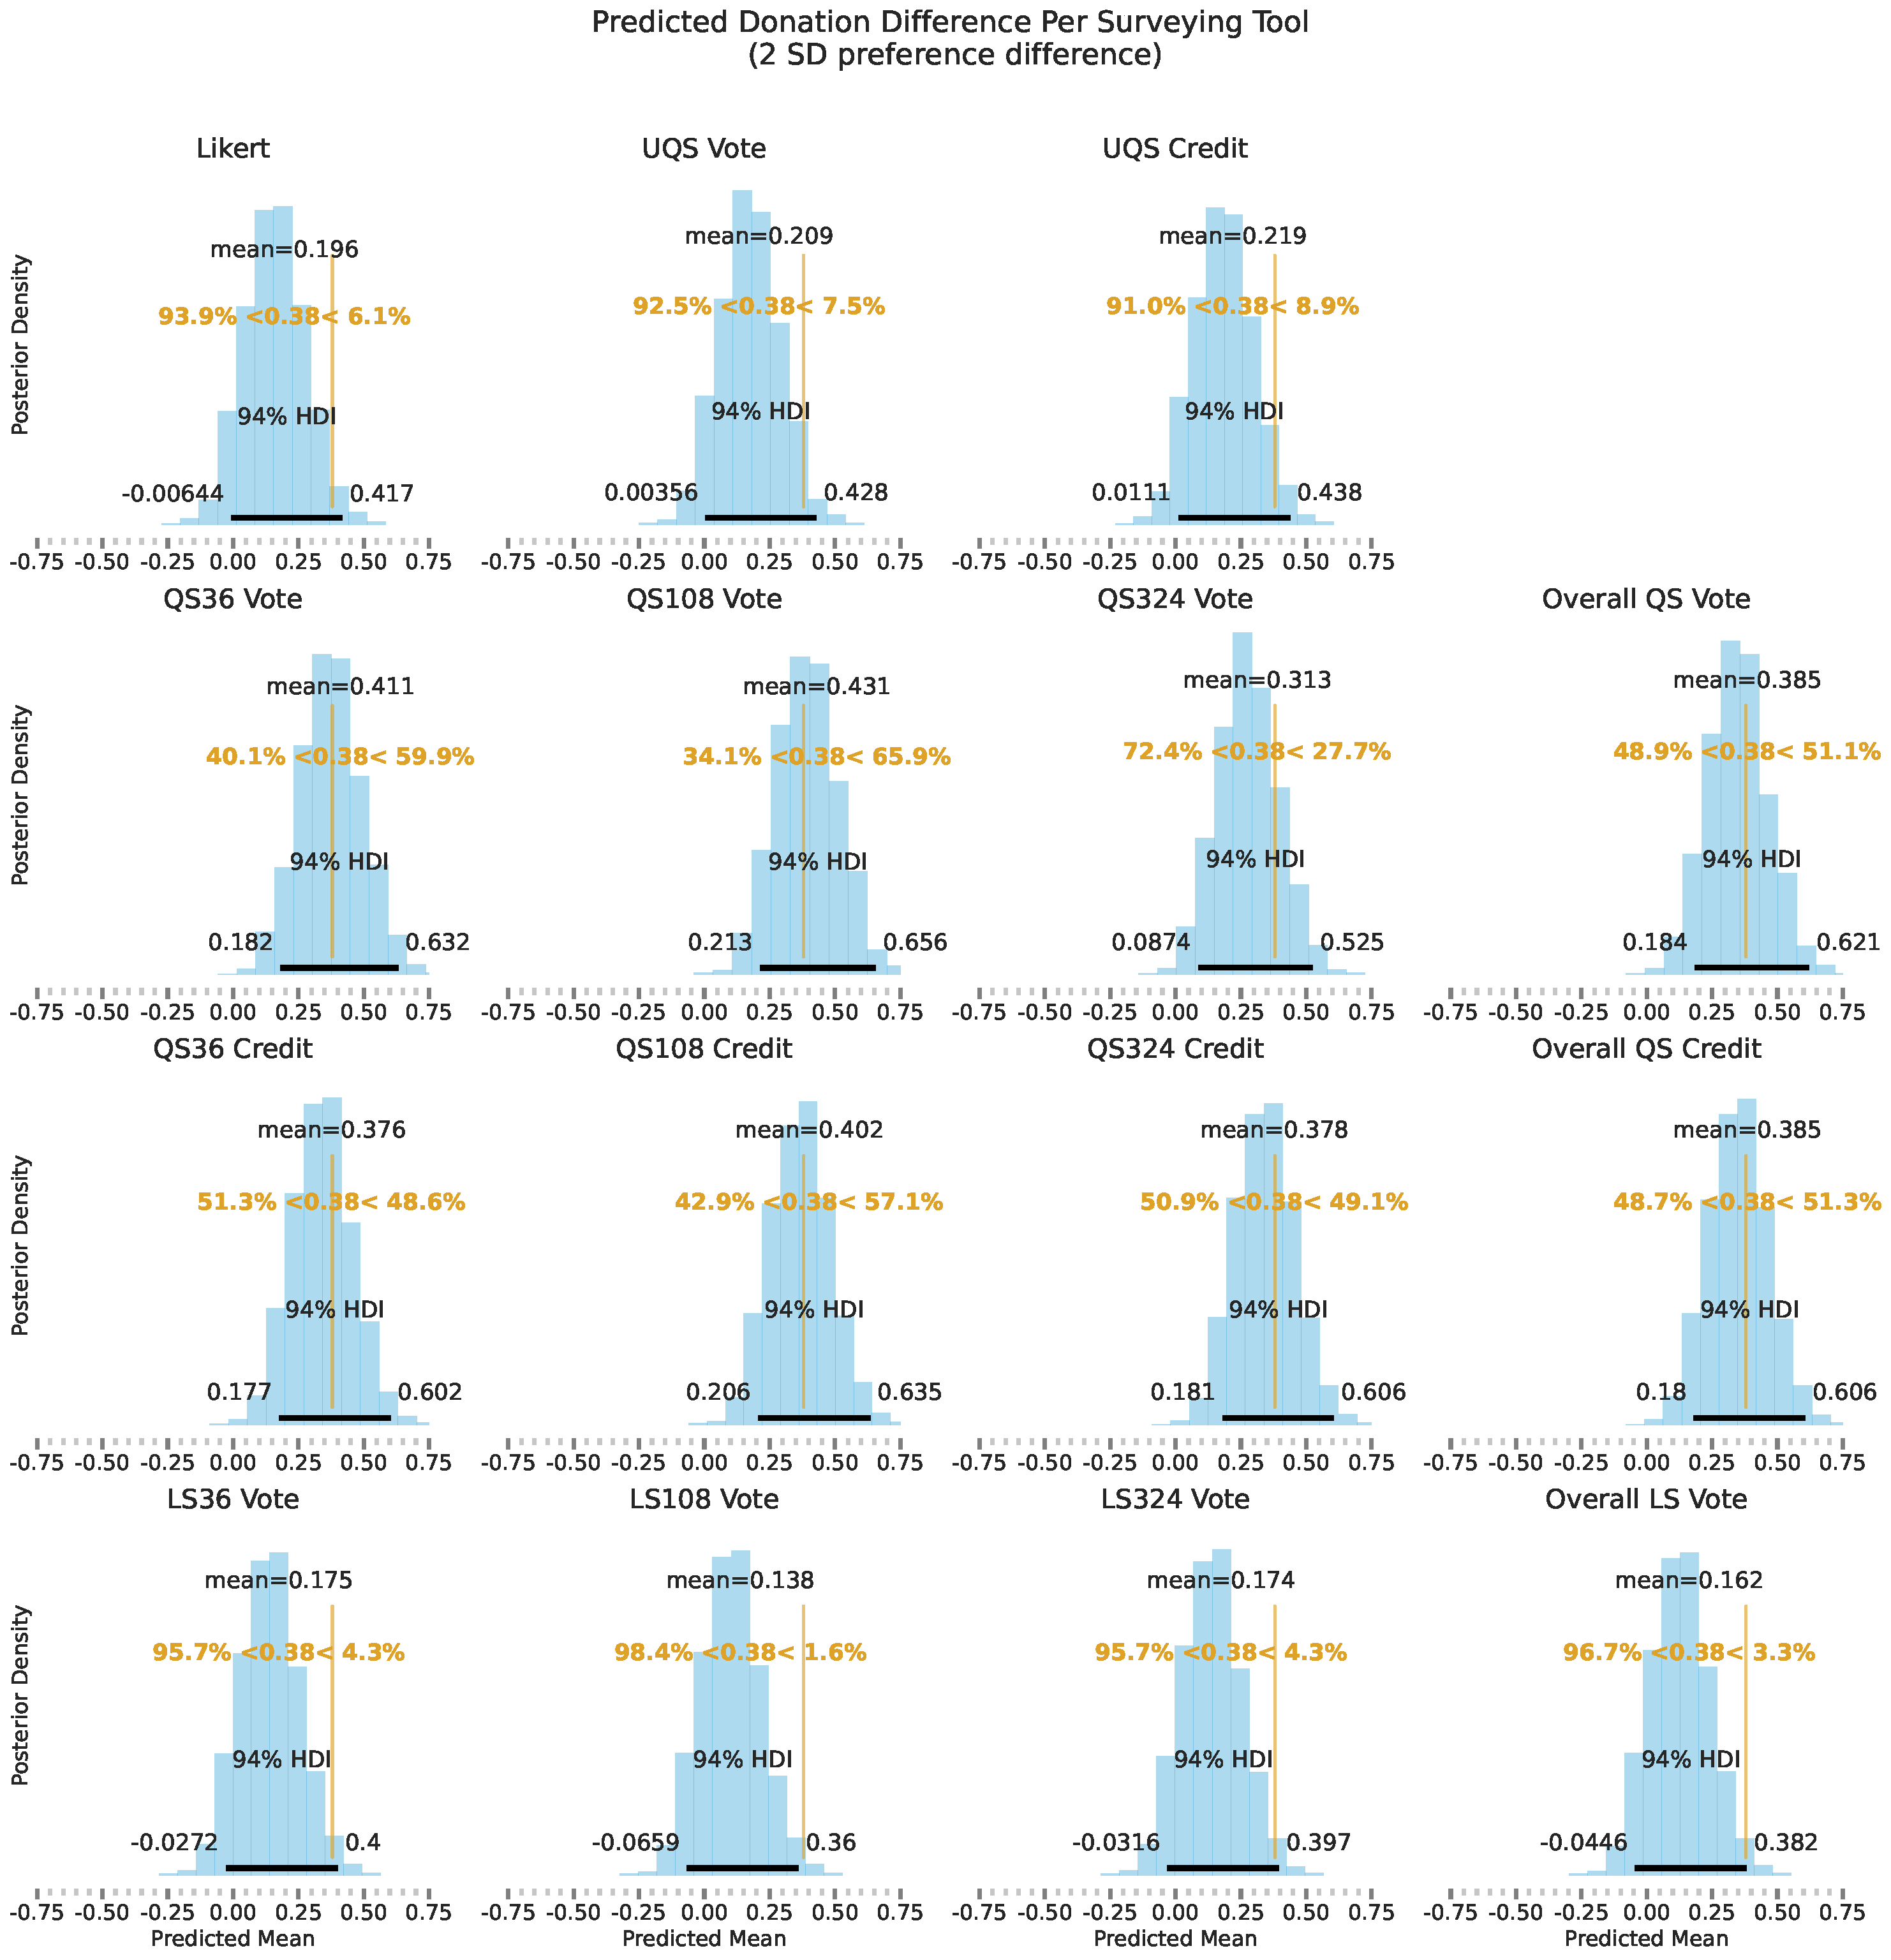
\includegraphics[width=\textwidth]{content/image/intensity_2sd.pdf}
    \caption{
    The posterior predictive distributions of donation differences for various surveying tools, assuming that the surveyed preference difference between two options is 2 standard deviations (SD) within our dataset's all pairwise differences. The x-axis displays predicted mean donation differences, while the y-axis represents posterior density, indicating the probability of various predicted mean donation differences occurring. The region indicated by the bolded black line represents the 94\% Highest Density Interval (HDI), providing the most credible range for the predicted donation difference. A vertical gold line at 0.38 reflects the ``perfect'' donation value corresponding to a 2 SD-surveyed preference difference. In this plot, aside from QS (votes and credit), other surveying tools produced donation predictions that fell short of the 0.38 threshold, suggesting that these tools overly expressed preference intensity rather than accurately capturing it.~\textbf{Main takeaway:} QS is capable of capturing the intensity of medium-sized (2 SD) preference differences between options accurately.
    }
    \label{fig:donation_posterior}
\end{figure*}


\textbf{Results interpretation:} With the fitted intensity model, we calculate the posterior predictive distribution of the mean of donation differences ($\mu_{\Delta_{\text{Predicted Donation}}}$), given a preference difference intensity between any two options elicited by a survey tool ($\Delta_{\text{Survey}}$). Three such distributions are constructed for each survey tool, one for a small, medium, and large preference difference elicited by the tool respectively (i.e., $\Delta_{\text{Survey}}$ = 0.19, 0.38, 0.57, corresponding to $median(\Delta_{\text{Survey}})+k \times std(\Delta_{\text{Survey}})$, where $k=1, 2, 3$). We then perform two comparison tasks using these posterior distributions of $\mu_{\Delta_{\text{Predicted Donation}}}$. 

First, we evaluate if predicted normalized donation differences $\Delta_{\text{Predicted Donation}}$ significantly differ from the ``perfect'' predicted donation difference ($\Delta_{\text{Donation Ref}}$). A predicted normalized donation difference between two options is ``perfect'' when it equals the normalized difference between the preferences elicited by the survey tool ($\Delta_{\text{Donation Ref}} = \Delta_{\text{Survey}}$). When $\Delta_{\text{Predicted Donation}} < \Delta_{\text{Donation Ref}}$, it means that our participants donated less to their preferred option than they said they would on the survey (relative to the less-preferred option), and vice-versa. We conclude that a survey tool failed to reflect a given preference difference intensity well when the 94\% Highest Posterior Density Interval (HPDI) of the distribution of $\mu_{\Delta_{\text{Predicted Donation}}}$ does not include $\Delta_{\text{Donation Ref}}$. 

Second, we compare the posterior distributions of $\mu_{\Delta_{\text{Predicted Donation}}}$ between survey conditions for the same $\Delta_{\text{Survey}}$. Such comparisons provide insights into how a survey tool performs relative to another. We construct the posterior distribution of Cohen's d to quantify the difference between the $\mu_{\Delta_{\text{Predicted Donation}}}$ of a pair of survey conditions. We report that a survey tool's ability to reflect a preference intensity differs from another when the 94\% HPDI of the Cohen's d distribution excludes zero. 

\textbf{Small $\Delta_{\text{Survey}}$ in all tested survey tools predicted $\Delta_{\text{Predicted Donation}}$ well.} Among them, Likert, UQS vote, UQS credit, and LS results aligned best with donation differences (mean of $\mu_{\Delta_{\text{Predicted Donation}}}$ = 0.15, 0.17, 0.18, 0.15, respectively; $\Delta_{\text{Donation Ref}}$ = 0.19). When participants expressed a small difference in QS vote and credit between two options, they expressed larger differences in donations (mean of $\mu_{\Delta_{\text{Predicted Donation}}}$ = 0.29, 0.26, respectively). But their donation differences did not differ significantly from the ``perfect'' difference ($\Delta_{\text{Donation Ref}}$ = 0.19).

\textbf{As $\Delta_{\text{Survey}}$ increased to medium and large sizes, only those elicited by QS (both vote and credit, regardless of the budget size) were well-reflected in the corresponding donation differences.} For instance, Figure~\ref{fig:donation_posterior} shows that when QS vote and credit $\Delta_{\text{Survey}} = 0.38$ (medium difference), the mean of $\mu_{\Delta_{\text{Predicted Donation}}} = 0.39$ (94\% HPDI for QS vote = [0.18, 0.62], for QS credit = [0.18, 0.61]). \textbf{Results from QS aligned significantly better with donation results than those from the Likert scale with a medium to large effect size}\footnote{Cohen's d = 0.2, 0.5, 0.8 corresponds to a small, medium, and large effect size, respectively}. Moreover, QS's advantage over the Likert scale increased with $\Delta_{\text{Survey}}$, as shown in Figure~\ref{fig:comparison}. Using the donation prediction accuracy of QS credit vs. Likert scale as an example, the mean Cohen's d increases from 0.71 to 0.99 when $\Delta_{\text{Survey}}$ changes from medium (Cohen's d 94\% HPDI = [0.62, 0.81]) to large (Cohen's d 94\% HPDI = [0.89, 1.09]).

\textbf{On the other hand, for medium and large $\Delta_{\text{Survey}}$, UQS (i.e., QS without a budget) predicted donation difference similarly to the Likert scale, hence significantly worse than QS. Furthermore, LS with various budget sizes (i.e., QS without the quadratic cost) performed worse than Likert and UQS with a small effect size.} When participants conveyed a medium-sized or larger preference difference between two options in Likert, UQS, or LS, they expressed a weaker difference in donations. A large $\Delta_{\text{Survey}}$ in Likert, UQS, and LS, for instance, predicted a mean $\mu_{\Delta_{\text{Predicted Donation}}}$ of 0.25, 0.25, and 0.17 respectively, far lower than the ideal difference ($\Delta_{\text{Donation Ref}}$ = 0.57).